\documentclass[12pt,a4paper]{report}
\usepackage{amssymb,amsthm,amsmath,amscd}
\usepackage{latexsym}
\usepackage{enumerate}
\usepackage[german]{babel}
\usepackage{verbatim}
\usepackage[hyphens]{url}
\usepackage{hyperref}
\usepackage[utf8]{inputenc}
\usepackage{pdfpages}
\usepackage{graphicx}
\usepackage{csquotes}
\usepackage[landscape]{geometry}
\begin{document}
\begin{titlepage}
	\begin{center}

		\vspace*{1.0cm}
		\huge
		\textsc{\bf{PS Algorithmen für verteilte Systeme}}

		\vspace*{4.0cm}
		\textsc{
			\normalsize{eingereicht von} \\[0.5\baselineskip]
			{\large Baumgartner Dominik, Dafir Samy}
		}

		\vspace*{3.0cm}
		\textsc{
			\normalsize{Gruppe  1(16:00)}
		}

	\end{center}
\end{titlepage}

\section*{Aufgabe 16}

\subsection*{Beschreibung:}
\textbf{Zugrundeliegendes Modell:}\\
 Hierbei wurde das Randomized-Rumorspreading-Modell verwendet. Gegeben ist ein Graph $G_t=(V,E_t \subseteq VxV)$ mit $t \ge 1$. In jeder Runde sucht sich eine Person $u \in V$ einen Kommunikationspartner $v \in V$ zufällig (unabhängig und gleich verteilt) aus und ruft diesen an. Eine Verbindung kann nur zwischen zwei benachbarten Knoten zustande kommen und eine Nachricht kann in beide Richtungen übermittelt werden. Zu beginn wir ein Gerücht verbreitet, Person $u$ kann nun entscheiden, ob die Person $v$ dieses Gerücht übermittelt unabhängig davon ob $v$ dies bereits kennt.\\
\\
\textbf{Modell I Karp:}\\
Verwenden den Median-Counter-Algorithmus, der $O(\ln(n))$ Runden benötigt um alle Knoten zu informieren und $O(n\ln(\ln(n)))$ Nachrichten sendet. Ob nun ein Knoten das Gerücht verbreitet oder nicht hängt vom Zustand des Knotens ab (address-oblivious: Knotenzustand unabhängig von den Adressen der Nachbarn aber abhängig von der Anzahl der Nachbarn). Dieser Algorithmus ist nun unabhängig von der Wahrscheinlichkeitsverteilung mit welcher die Nachbarn ausgewählt werden, sofern jeder Knoten unabhängig agiert und die selben Wahrscheinlichkeitsverteilungen verwendet. Es wird außerdem die generell niedrigere untere Schranken von $\Omega (n ln(\ln(n)))$ Übertragungen gezeigt. Der Algorithmus besitzt vier verschiedene Zustände: A,B,C und D. Zustand A bedeutet, dass der Knoten noch uninformiert ist. In jedem anderen Zustand besitzt der Knoten bereits das Gerücht. Wenn sich der Knoten in Zustand B oder C befindet, dann pusht\&pullt er das Gerücht zum jeweiligen verbundenen Knoten. In Zustand D verbreitet der Knoten das Gerücht nicht mehr. \\
Knoten im Zustand A:
bekommt ein solcher Knoten nun ein Gerücht von einem Knoten mit Zustand B, dann wechselt er von A nach B-1 (1...counter). Bekommt er es von einem Knoten mit Zustand C, dann wechselt er nach Zustand C.\\
Knoten im Zustand B-$m$: Median Regel: Wenn ein Knoten im Zustand B-$m$ mehr Gerüchte gesendet bekommt als Knoten im Zustand B-$m'$ mit $m' \ge m$ sind, als Knoten im Zustand A und B-$m''$ mit $m'' < m$, dann wechselt er auf Zustand B-$(m+1)$. Ausnahme dann, wenn der counter sein Maximum erreicht hat ($O(\ln(\ln(n)))$), dann wechselt er auf Zustand C. Der Knoten wechselt auch auf Zustand C, wenn er das Gerücht von einem Knoten im Zustand C bekommt.\\
Knoten im Zustand C: Knoten bleiben für $O(\ln(\ln(n)))$ Runden in diesem Zustand und wechseln dann auf D.
\\
\\
\textbf{Modell II Doerr:}\\
Verwende ein Quasi-Random-Modell. Jeder Knoten besitz eine zyklische Liste an Nachbarn. Wenn ein Knoten informiert wird, sucht sich dieser in der nächsten Runde einen Nachbarn aus seiner Liste aus. In jeder darauffolgenden Runde sendet dieser Knoten weiter Nachrichten an die Nachbarknoten in der Reihenfolge seiner Liste. Daraus folgt, dass alle Knoten in $d(G)$ informiert werden. Dieser Algorithmus besitzt eine $O(\log(n))$ Laufzeitgrenze welche auch für sparse connected random graphs mit $p=\frac{\log(n)+\omega(1)}{n}$ und einer unteren Schranke von $\Omega(\log^2(n))$ gilt, sodass mit Wahrscheinlichkeit $1-n^{-1}$ alle Knoten informiert werden. Betrachten auch sog. Expanding-Graphs mit 3 Eigenschaften:\\
Eigenschaft 1: Knotenexpansion von nicht zu großen Teilmengen\\
Eigenschaft 2: Kantenexpansion\\
Eigenschaft 3: Regularität des Graphen
\\
\\
\textbf{Modell III Elsässer:}\\
Es gibt zwei Modelle: Modell 1: Zu Beginn ein Gerücht. In jeder Runde stellt ein Knoten eine Verbindung mit vier seiner Nachbarn her. Knotenzustände: A active, U uninformed, G going down, S sleeping. Wenn der Knoten den Zustand A oder G besitzt, schickt dieser das Gerücht und dessen Alter an alle vier ausgewählten Knoten weiter und er kann von den anderen Knoten das Gerücht erhalten. Ein Knoten wechselt von Zustand U nach A, wenn dieser ein Gerücht bekommt.
Von Zustand A nach G, wenn das Alter $>\log_9(n)$ ist und von G nach S, wenn $counter = a*\log(\log(n))$ ist. Nachrichten können in beide Richtungen versendet werden.\\
Modell 2: Auch hier zu Beginn ein Gerücht. In jeder Runde wählt Knoten $u$ einen seiner Nachbarn aus einer Liste der nicht gewählten Nachbarn in $t-((t-1)mod(4))$ Schritten und stellt eine Verbindung zu ihm her. Wechselt von Zustand A nach G, wenn das Alter des Gerüchts $\ge \log_3(n)$ ist. Nachrichten können in beide Richtungen versendet werden.\\
Wenn nun $p>\frac{\log^{\delta}(n)}{n}$, mit $\delta$ passend gewählt, ist die Anzahl der Runden $O(\log(n))$ und $O(n\log(\log(n)))$ Nachrichten.
\\
\\
\textbf{Eigene Einschätzung:} Unserer Meinung nach ist jener Algorithmus von Modell II am besten, der nicht die gleichen, bereits kontaktierten Knoten auswählt und somit alle Knoten in $d(G)$ informiert werden. Danach kommt der Algorithmus von Modell III, da dieser entweder 4 Knoten gleichzeitig kontaktiert bzw. Knoten die schon länger nicht mehr kontaktiert wurden kontaktiert. Zum Schluss kommt der Algorithmus von Modell I, jedoch nur weil dieser Knoten zufällig auswählt und damit potentiell Knoten mehrfach hintereinander informiert, bevor alle Nachbarn durchlaufen wurden.

\subsection*{Implementierung:}
Für diesen Teil wurde der Rumor-Spreading Algorithmus (Model I) nach Elsässer und Sauerwald implementiert und empirisch hinsichtlich Laufzeit (Runden) und versendeten Nachrichten ausgewertet. Der implementierte Algorithmus wurde auf einem 
Zufallsgraphen $G_{n,p}$ mit n = 10000 und p = 0.005 getestet.
Der Publikation \"The Power of Memory in Randomized Broadcasting\" zufolge kann dieser Algorithmus alle Knoten in einem
Graphen innerhalb $O(ln(n))$ Runden und mit $O(n * log(log(n)))$ Nachrichten informieren.\\
Unsere empirischen Untersuchungen lassen auf die obigen Laufzeiten schließen.
Dazu wurde die Informationsverteilung auf 300 zufällig erstellten Graphen mit obigen Eigenschaften ausgeführt.
Um eine zufällige Übereinstimmung der Laufzeit mit Gaphen der Größe 10000 auszuschließen wurde der Algorithmus
zusätzlich auf 40 Zufallsgraphen der Größe 100000 angewandt. Auch dies ergab eine Übereinstimmung mit der asymptotischen
Laufzeit des Algorithmus. Im folgenden werden nun 2 Graphen gezeigt, die die Laufzeiten und Nachrichtenanzahlen für 10000, sowie 100000 Knoten zeigen.

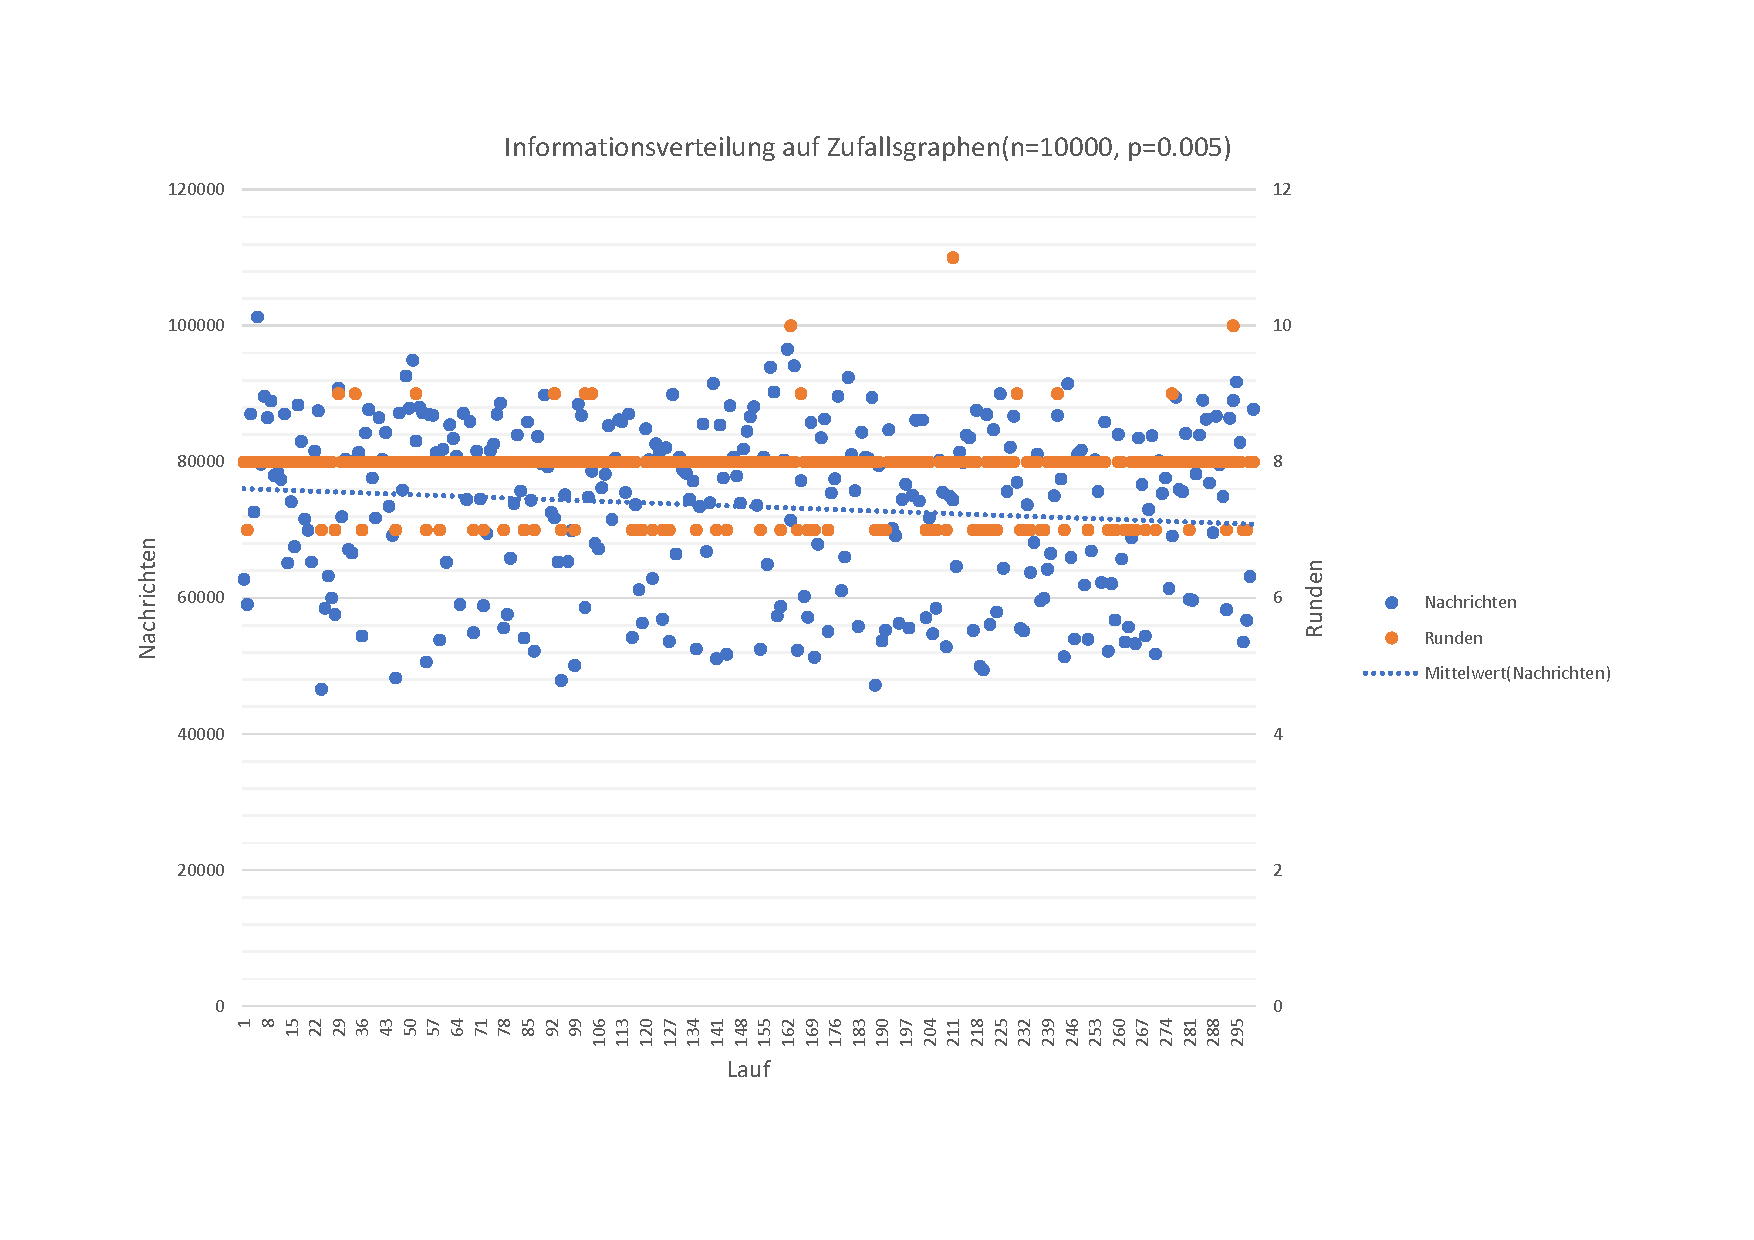
\includepdf{10000.pdf}
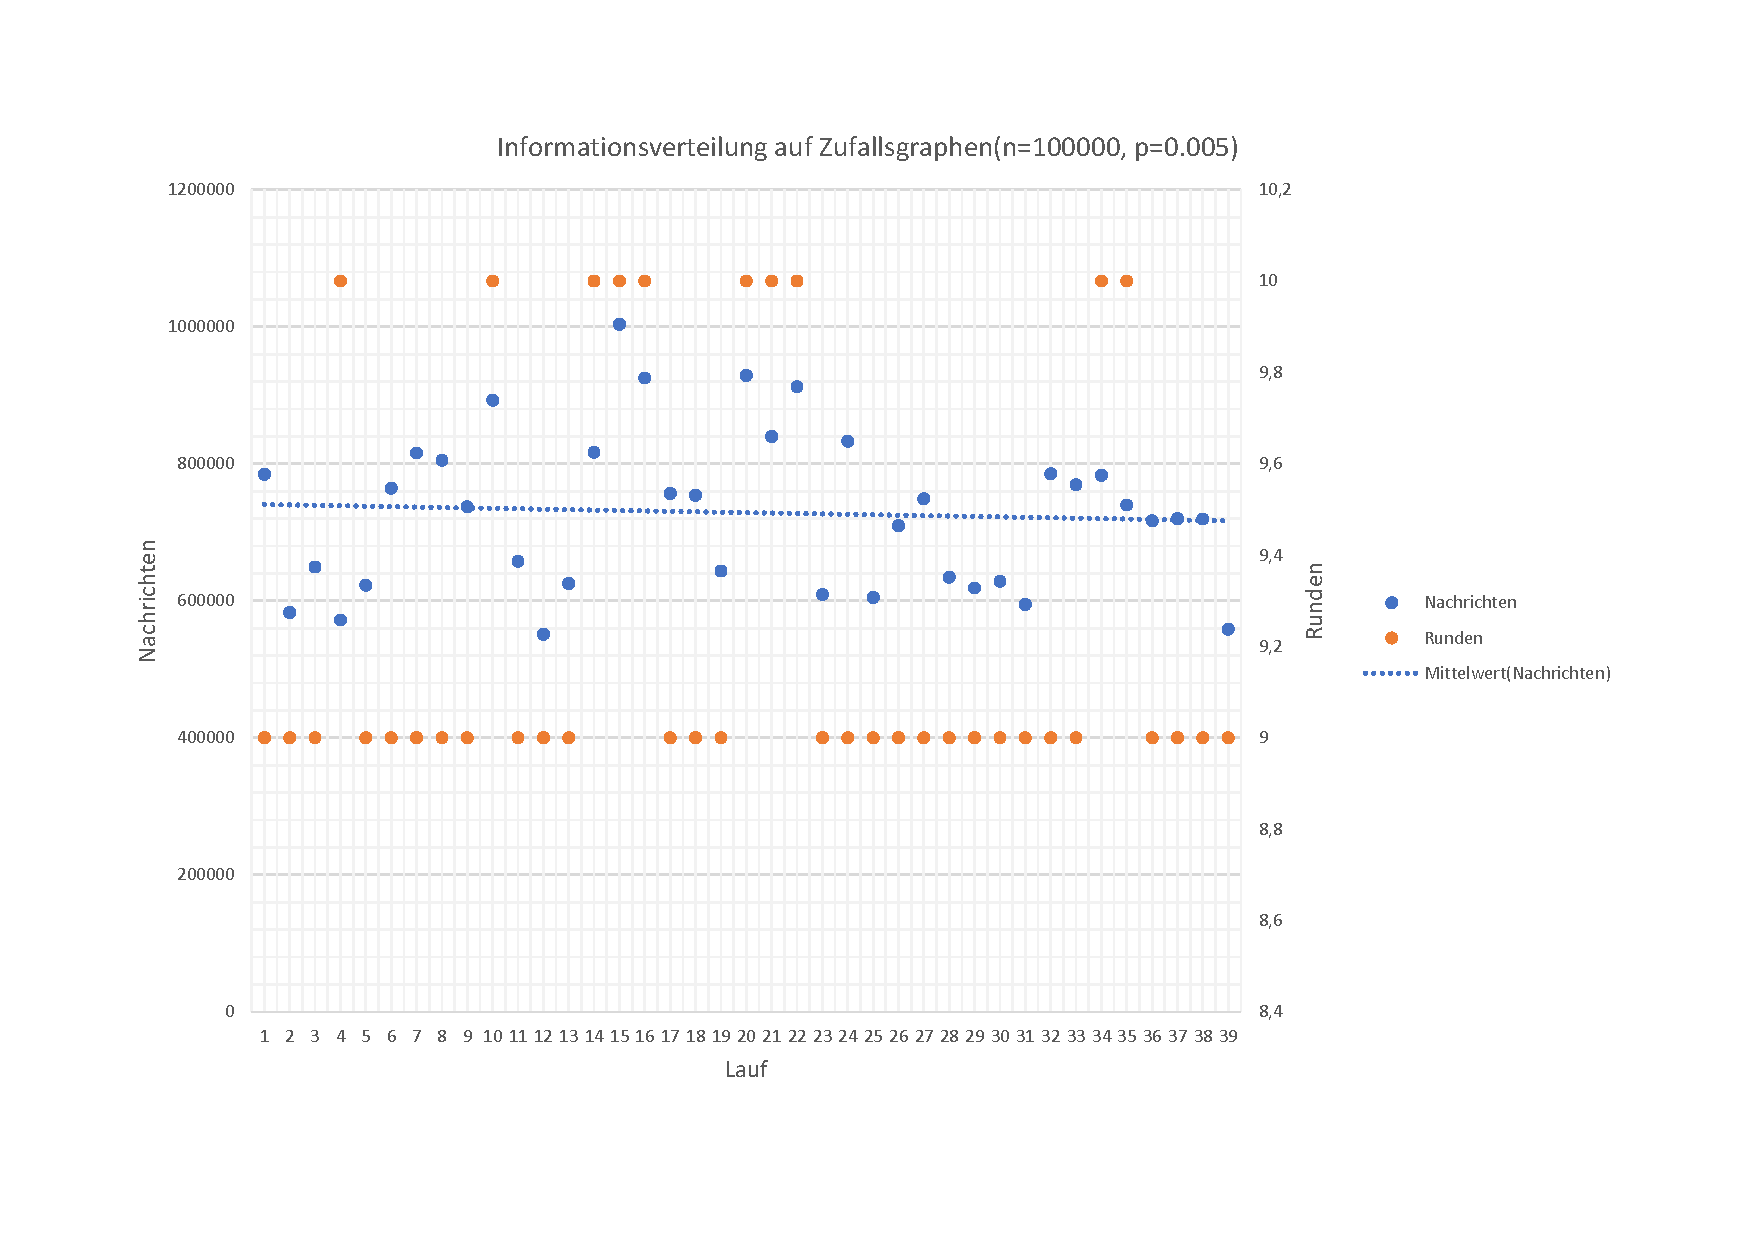
\includepdf{100000.pdf}

\end{document}